\section{IV. Thống kê mô tả}
\label{iv.-thux1ed1ng-kuxea-muxf4-tux1ea3}

\subsection{1. Tạo function và lập bảng tính thống kê mô tả cho các biến liên tục:}

\begin{Shaded}
\begin{Highlighting}[]
\NormalTok{conts\_var }\OtherTok{\textless{}{-}}\NormalTok{ data[, }\FunctionTok{c}\NormalTok{(}\StringTok{"layer\_height"}\NormalTok{, }\StringTok{"wall\_thickness"}\NormalTok{, }\StringTok{"infill\_density"}\NormalTok{, }
                      \StringTok{"nozzle\_temperature"}\NormalTok{, }\StringTok{"bed\_temperature"}\NormalTok{, }\StringTok{"print\_speed"}\NormalTok{, }
                      \StringTok{"fan\_speed"}\NormalTok{, }\StringTok{"roughness"}\NormalTok{)] }
\end{Highlighting}
\end{Shaded}

Trong bảng gồm các giá trị.

\begin{Shaded}
\begin{Highlighting}[]
\NormalTok{mean\_val }\OtherTok{\textless{}{-}} \FunctionTok{apply}\NormalTok{(conts\_var, }\DecValTok{2}\NormalTok{, mean)}
\NormalTok{sd\_val }\OtherTok{\textless{}{-}} \FunctionTok{apply}\NormalTok{(conts\_var, }\DecValTok{2}\NormalTok{, sd)}
\NormalTok{var\_val }\OtherTok{\textless{}{-}} \FunctionTok{apply}\NormalTok{(conts\_var, }\DecValTok{2}\NormalTok{, var)}
\NormalTok{median\_val }\OtherTok{\textless{}{-}} \FunctionTok{apply}\NormalTok{(conts\_var, }\DecValTok{2}\NormalTok{, median)}
\NormalTok{min\_val }\OtherTok{\textless{}{-}} \FunctionTok{apply}\NormalTok{(conts\_var, }\DecValTok{2}\NormalTok{, min)}
\NormalTok{max\_val }\OtherTok{\textless{}{-}} \FunctionTok{apply}\NormalTok{(conts\_var, }\DecValTok{2}\NormalTok{, max)}
\NormalTok{quantile1 }\OtherTok{\textless{}{-}} \FunctionTok{apply}\NormalTok{(conts\_var, }\DecValTok{2}\NormalTok{, }\ControlFlowTok{function}\NormalTok{(x) }\FunctionTok{quantile}\NormalTok{(x, }\AttributeTok{probs =} \FloatTok{0.25}\NormalTok{))}
\NormalTok{quantile3 }\OtherTok{\textless{}{-}} \FunctionTok{apply}\NormalTok{(conts\_var, }\DecValTok{2}\NormalTok{, }\ControlFlowTok{function}\NormalTok{(x) }\FunctionTok{quantile}\NormalTok{(x, }\AttributeTok{probs =} \FloatTok{0.75}\NormalTok{))}
\CommentTok{\#Trung bình, độ lệch chuẩn, biến số, trung vị, GTNN, GTLN, phân vị đơn, phân vị 3}

\NormalTok{summary\_stats }\OtherTok{\textless{}{-}} \FunctionTok{data.frame}\NormalTok{(}\AttributeTok{mean =}\NormalTok{ mean\_val, }\AttributeTok{sd =}\NormalTok{ sd\_val, }\AttributeTok{var =}\NormalTok{ var\_val, }
                            \AttributeTok{median =}\NormalTok{ median\_val, }\AttributeTok{min =}\NormalTok{ min\_val, }\AttributeTok{max =}\NormalTok{ max\_val, }
                            \AttributeTok{quantile1 =}\NormalTok{ quantile1, }\AttributeTok{quantile3 =}\NormalTok{ quantile3)}
\NormalTok{knitr}\SpecialCharTok{::}\FunctionTok{kable}\NormalTok{(}\FunctionTok{t}\NormalTok{(summary\_stats))}
\end{Highlighting}
\end{Shaded}

{\def\LTcaptype{none} % do not increment counter
\begin{longtable}[]{@{}
  >{\raggedright\arraybackslash}p{(\linewidth - 16\tabcolsep) * \real{0.0820}}
  >{\raggedleft\arraybackslash}p{(\linewidth - 16\tabcolsep) * \real{0.1066}}
  >{\raggedleft\arraybackslash}p{(\linewidth - 16\tabcolsep) * \real{0.1230}}
  >{\raggedleft\arraybackslash}p{(\linewidth - 16\tabcolsep) * \real{0.1230}}
  >{\raggedleft\arraybackslash}p{(\linewidth - 16\tabcolsep) * \real{0.1557}}
  >{\raggedleft\arraybackslash}p{(\linewidth - 16\tabcolsep) * \real{0.1311}}
  >{\raggedleft\arraybackslash}p{(\linewidth - 16\tabcolsep) * \real{0.0984}}
  >{\raggedleft\arraybackslash}p{(\linewidth - 16\tabcolsep) * \real{0.0902}}
  >{\raggedleft\arraybackslash}p{(\linewidth - 16\tabcolsep) * \real{0.0902}}@{}}
\toprule\noalign{}
\begin{minipage}[b]{\linewidth}\raggedright
\end{minipage} & \begin{minipage}[b]{\linewidth}\raggedleft
layer \_height
\end{minipage} & \begin{minipage}[b]{\linewidth}\raggedleft
wall \_thickness
\end{minipage} & \begin{minipage}[b]{\linewidth}\raggedleft
infill \_density
\end{minipage} & \begin{minipage}[b]{\linewidth}\raggedleft
nozzle \_temperature
\end{minipage} & \begin{minipage}[b]{\linewidth}\raggedleft
bed \_temperature
\end{minipage} & \begin{minipage}[b]{\linewidth}\raggedleft
print \_speed
\end{minipage} & \begin{minipage}[b]{\linewidth}\raggedleft
fan \_speed
\end{minipage} & \begin{minipage}[b]{\linewidth}\raggedleft
roughness
\end{minipage} \\
\midrule\noalign{}
\endhead
\bottomrule\noalign{}
\endlastfoot
mean & 0.1060000 & 5.220000 & 53.40000 & 221.50000 & 70.000000 & 64.0000
& 50.00000 & 170.58000 \\
sd & 0.0643967 & 2.922747 & 25.36348 & 14.82035 & 7.142857 & 29.6923 &
35.71429 & 99.03413 \\
var & 0.0041469 & 8.542449 & 643.30612 & 219.64286 & 51.020408 &
881.6327 & 1275.5102 & 9807.75878 \\
median & 0.1000000 & 5.000000 & 50.00000 & 220.00000 & 70.000000 &
60.0000 & 50.00000 & 165.50000 \\
min & 0.0200000 & 1.000000 & 10.00000 & 200.00000 & 60.000000 & 40.0000
& 0.00000 & 21.00000 \\
max & 0.2000000 & 10.000000 & 90.00000 & 250.00000 & 80.000000 &
120.0000 & 100.00000 & 368.00000 \\
quantile1 & 0.0600000 & 3.000000 & 40.00000 & 210.00000 & 65.000000 &
40.0000 & 25.00000 & 92.00000 \\
quantile3 & 0.1500000 & 7.000000 & 80.00000 & 230.00000 & 75.000000 &
60.0000 & 75.00000 & 239.25000 \\
\end{longtable}
}

\subsection{2. Vẽ đồ thị histogram thể hiện phân phối cho biến
\texttt{roughness}:}

\begin{Shaded}
\begin{Highlighting}[]
\FunctionTok{hist}\NormalTok{(new\_data}\SpecialCharTok{$}\NormalTok{roughness, }\AttributeTok{xlab =} \StringTok{"Roughness"}\NormalTok{, }\AttributeTok{ylab =} \StringTok{"Number of Samples"}\NormalTok{, }
\AttributeTok{main =}\StringTok{"Histogram roughness"}\NormalTok{,} \AttributeTok{col =} \StringTok{"lightyellow"}\NormalTok{, }\AttributeTok{labels =} \ConstantTok{TRUE}\NormalTok{, }\AttributeTok{ylim =} \FunctionTok{c}\NormalTok{(}\DecValTok{0}\NormalTok{, }\DecValTok{12}\NormalTok{))}
\end{Highlighting}
\end{Shaded}

\begin{figure}[htbp]
    \centering
    % Lệnh chèn ảnh gốc do R xuất ra
    \pandocbounded{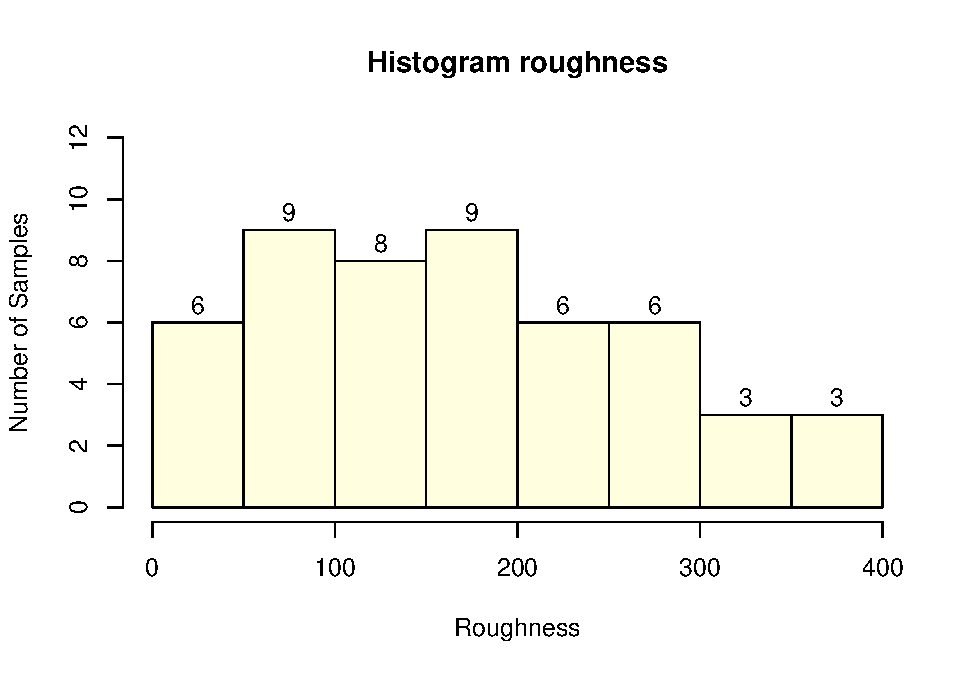
\includegraphics[keepaspectratio]{unnamed-chunk-6-1.pdf}}
    
    % Chú thích hình ảnh (bắt buộc để vào Danh sách hình vẽ)
    \caption{Biểu đồ Histogram thể hiện phân phối của độ nhám bề mặt (roughness)}
    
    % Nhãn để trích dẫn chéo trong bài (Ví dụ: xem Hình \ref{fig:hist_roughness})
    \label{fig:hist_roughness}
\end{figure}
\newpage

\textbf{Nhận xét:}

\begin{itemize}
\tightlist
\item
  Đồ thị phân phối hơi lệch về phải, không có phân phối chuẩn.
\item
  Phân bố tần số cao nhất trong khoảng (50-200), và thấp nhât trong
  khoảng (300-400).
\end{itemize}

\subsection{3. Vẽ các đồ thị boxplot thể hiện phân phối của biến roughness theo các biến phân loại.}

\subsubsection{3.1. Biểu đồ hộp so sánh \texttt{độ\ nhám} giữa các loại biến mật độ mô hình:}

\begin{Shaded}
\begin{Highlighting}[]
\FunctionTok{boxplot}\NormalTok{(roughness }\SpecialCharTok{\textasciitilde{}}\NormalTok{ infill\_pattern, }\AttributeTok{data =}\NormalTok{ new\_data, }\AttributeTok{col =} \FunctionTok{c}\NormalTok{(}\StringTok{"red"}\NormalTok{, }\StringTok{"lightblue"}\NormalTok{),}
        \AttributeTok{main =} \StringTok{"Boxplot roughness theo infill\_pattern"}\NormalTok{)}
\end{Highlighting}
\end{Shaded}

\begin{figure}[htbp]
    \centering
    \pandocbounded{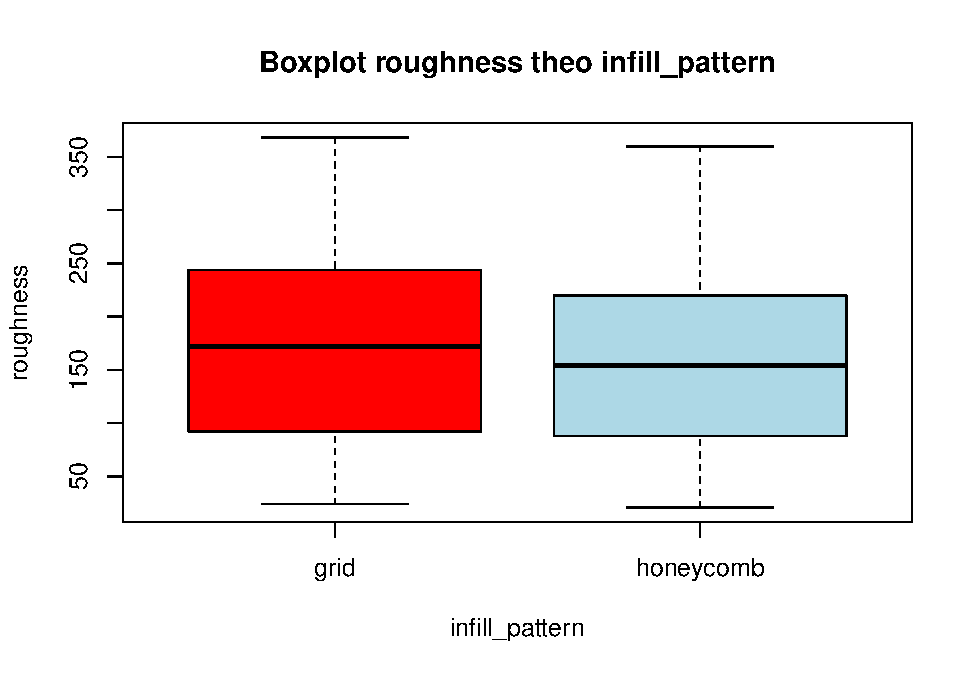
\includegraphics[keepaspectratio]{unnamed-chunk-7-1.pdf}}
    \caption{Biểu đồ Boxplot phân bố độ nhám theo kiểu điền đầy (infill pattern)}
    \label{fig:box_infill}
\end{figure}
\newpage

\textbf{Nhận xét:} Không có sự khác biệt nhiều về phân phối của
\texttt{độ\ nhám} ở 2 nhóm \texttt{infill\_pattern}, ta dự đoán yếu tố
\texttt{infill\_pattern} không ảnh hưởng đến độ.

\subsubsection{3.2. Biểu đồ hộp so sánh \texttt{độ\ nhám} theo
\texttt{vật\ liêu}:}

\begin{Shaded}
\begin{Highlighting}[]
\FunctionTok{boxplot}\NormalTok{(roughness }\SpecialCharTok{\textasciitilde{}}\NormalTok{ material, }\AttributeTok{data =}\NormalTok{ new\_data, }\AttributeTok{col =} \FunctionTok{c}\NormalTok{(}\StringTok{"red"}\NormalTok{, }\StringTok{"lightblue"}\NormalTok{),}
        \AttributeTok{main =} \StringTok{"Boxplot roughness theo material"}\NormalTok{)}
\end{Highlighting}
\end{Shaded}

\begin{figure}[htbp]
    \centering
    \pandocbounded{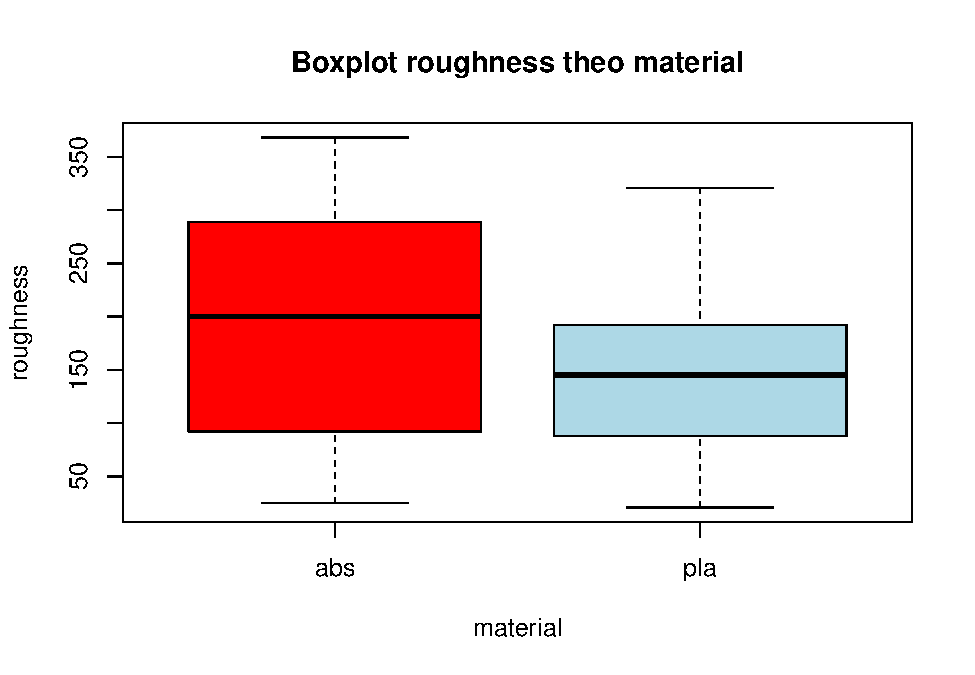
\includegraphics[keepaspectratio]{unnamed-chunk-8-1.pdf}}
    \caption{Biểu đồ Boxplot phân bố độ nhám theo loại vật liệu (ABS và PLA)}
    \label{fig:box_material}
\end{figure}
\newpage

\textbf{Nhận xét:}

\begin{itemize}
\tightlist
\item
  Nhìn chung sự phân phối của 2 nhóm \texttt{material} cũng tương đồng
  nhưng ở loại vật liệu \texttt{abs} thì có độ nhám tối đa cao hơn loại
  vật liệu \texttt{pla}.
\item
  Về khoảng phân bố thì loại vật liệu \texttt{pla} thấp hơn so với loại
  vật liệu \texttt{abs}, ta dự đoán yếu tố material có ảnh hưởng đến
  biến phụ thuộc \texttt{roughness}.
\end{itemize}

\subsubsection*{3.3. Biểu đồ phân tán \texttt{chiều cao lớp in} và \texttt{độ nhám}:}

\begin{Shaded}
\begin{Highlighting}[]
\FunctionTok{plot}\NormalTok{(new\_data}\SpecialCharTok{$}\NormalTok{layer\_height, new\_data}\SpecialCharTok{$}\NormalTok{roughness, }\AttributeTok{col =} \StringTok{"blue"}\NormalTok{, }\AttributeTok{pch =} \DecValTok{15}\NormalTok{,}
     \AttributeTok{xlab =} \StringTok{"layer\_height"}\NormalTok{, }\AttributeTok{ylab =} \StringTok{"roughness"}\NormalTok{, }\AttributeTok{main =} \StringTok{"Scatter: layer\_height vs roughness"}\NormalTok{)}
\end{Highlighting}
\end{Shaded}

\begin{figure}[htbp]
    \centering
    \pandocbounded{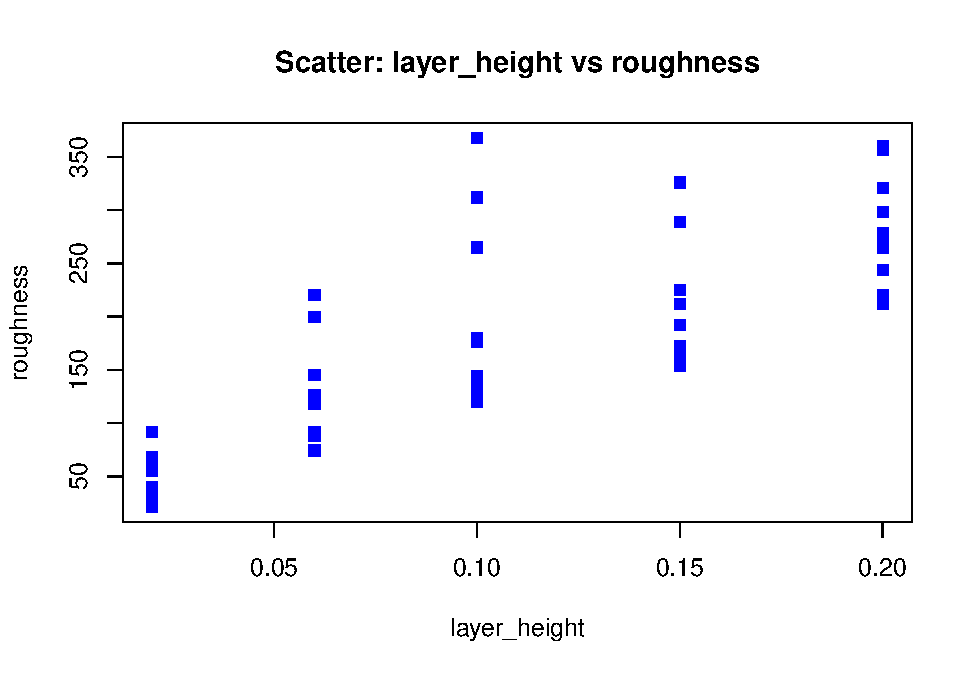
\includegraphics[keepaspectratio]{unnamed-chunk-9-1.pdf}}
    \caption{Biểu đồ phân tán (Scatter plot) giữa chiều cao lớp in và độ nhám}
    \label{fig:scatter_layer_roughness}
\end{figure}

\textbf{Nhận xét:}

\begin{itemize}
\tightlist
\item
  Các điểm phân bố có xu hướng tăng lên khi biến \texttt{layer\_height}
  tăng dần.
\item
  Các điểm không nằm quá sát nhau trên cùng 1 đường thẳng\\
\(\Rightarrow\) Có thể có quan hệ tuyến tính với nhau nhưng sẽ chỉ ở mức độ trung
  bình\\
 \(\Rightarrow\) Khi biến \texttt{layer\_height} thay đổi thì biến \texttt{roughness}
  cũng thay đổi theo hay nói cách khác, biến \texttt{layer\_height} có
  ảnh hưởng đến biến \texttt{roughness}.
\end{itemize}
\newpage